\chapter{Variational Quantum Eigensolver}
\mccorrect{[Insert introductory paragraph]}

\section{Variational Principle}

\section{Exponential Excitation Operators}
Recalling the Jordan-Wigner encoding for the creation and annhilation operators,
\begin{equation*}
    \hat a_j^+ = \frac{1}{2} (X - iY) \otimes Z^\rightarrow_{j-1} \qquad
    \hat a_j = \frac{1}{2} (X + iY) \otimes Z^\rightarrow_{j-1}
\end{equation*}
The anti-Hermitian fermionic single and double excitation operators $\kappa_p^q$ and $\kappa_{pq}^{rs}$
\begin{align*}
    F_p^q = \frac{i}{2} & (Y_p X_q - X_p Y_q) \prod_{k=p+1}^{q-1} Z_k \\
    %
    F_{pq}^{rs} = \frac{i}{8} (
      & X_p X_q Y_s X_r +
        Y_p X_q Y_s Y_r +
        X_p Y_q Y_s Y_r +
        X_p X_q X_s Y_r - \\
      & Y_p X_q X_s X_r -
        X_p Y_q X_s X_r -
        Y_p Y_q Y_s X_r -
        Y_p Y_q X_s Y_r )
    \prod_{k=p+1}^{q-1} Z_k
    \prod_{l=r+1}^{s-1} Z_l
\end{align*}
Multiplying by $\theta$ and exponentiating yields the parametrised unitary qubit operators,
\begin{equation*}
    U^q_p (\theta) =
    \text{exp} \left( i
    \frac{\theta}{2} (Y_p X_q - X_p Y_q) \prod_{k=p+1}^{q-1} Z_k \right)
\end{equation*}

\begin{equation*}
    U^{rs}_{pq} (\theta) = \text{exp} \left( i \frac{\theta}{8} (
    X_p X_q Y_s X_r
    + \dots -
    Y_p Y_q Y_s X_r -
    Y_p Y_q X_s Y_r )
    \prod_{k=p+1}^{q-1} Z_k
    \prod_{l=r+1}^{s-1} Z_l
    \right)
\end{equation*}
To summarise, we constructed anti-Hermitian single and double excitation operators from a linear combination of fermionic excitation operators,
\begin{equation*}
    \hat\kappa_p^q = a_q^\dagger a_p - a_p^\dagger a_q \qquad
    %
    \hat\kappa_{pq}^{rs} =
    a_r^\dagger a_s^\dagger a_q a_p - a_p^\dagger a_q^\dagger a_s a_r
\end{equation*}\smallskip
We then mapped these to qubit operators using the Jordan-Wigner transformation,
\begin{equation*}
    \hat\kappa_p^q \xrightarrow{\text{JW}} F_p^q \qquad\qquad
    \hat\kappa_{pq}^{rs} \xrightarrow{\text{JW}} F_{pq}^{rs}
\end{equation*}
And finally, we exponentiated to yield the parametrised unitary qubit operators.
\begin{equation*}
    U^q_p (\theta) = e^{\theta^q_p F_p^q} \qquad
    %
    U^{rs}_{pq}(\theta) = e^{\theta_{pq}^{rs} F_{pq}^{rs}}
\end{equation*}

Let's look again at the parametrised single-body unitary operator,
\begin{equation*}
\begin{gathered}
    U^q_p (\theta) =
    \text{exp} \left( i
    \frac{\theta}{2} (Y_p X_q - X_p Y_q) \prod_{k=p+1}^{q-1} Z_k \right) \\
    %
    U^q_p (\theta) =
    \left( \text{exp} \left[
    i \frac{\theta}{2} Y_p X_q \prod_{k=p+1}^{q-1} Z_k \right] \right)
    %
    \left( \text{exp} \left[ -
    i \frac{\theta}{2} X_p Y_q \prod_{k=p+1}^{q-1} Z_k \right] \right)
\end{gathered}
\end{equation*}

The first exponential term can be implemented by the following phase gadget.
\begin{equation*}
    \text{exp} \left( i
    \frac{\theta}{2} Y_p X_q \prod_{k=p+1}^{q-1} Z_k \right)
\end{equation*}

\begin{figure}[H]
\centering
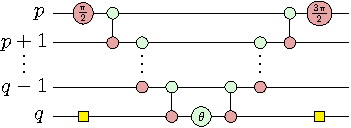
\includegraphics[width=8cm]{chapter-3/yx_cnot}
\end{figure}

Left CNOT ladder construction calculates the parity of the qubit state, and applies a rotation in the $Z$ basis if the parity is odd.

Whilst the second exponential term can be implemented by the phase gadget.
\begin{equation*}
    \text{exp} \left( - i
    \frac{\theta}{2} X_p Y_q \prod_{k=p+1}^{q-1} Z_k \right)
\end{equation*}

\begin{figure}[H]
\centering
    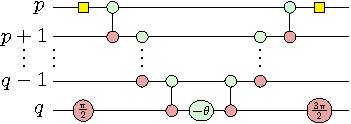
\includegraphics[width=8cm]{chapter-3/xy_cnot}
\end{figure}

%%% ----- %%%

Together, they constitute the single-body unitary excitation operator $U^q_p (\theta)$

\begin{figure}[H]
\centering
    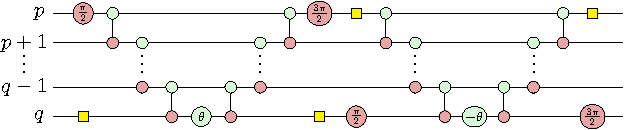
\includegraphics[width=14cm]{chapter-3/full_cnot}
\end{figure}

By defining the ordering of spin-orbitals such that adjacent spin-orbitals share the same spatial orbital, adjacent single-body operators commute.

\begin{equation*}
    \left[ \hat\kappa_p^q, \hat\kappa_{p+1}^{q+1} \right] = 0
\end{equation*}\smallskip

The same is therefore true for the resulting qubit operators,

\begin{equation*}
\begin{gathered}
    \left[ F_p^q, F_{p+1}^{q+1} \right] = 0 \\
    p, q \in \text{even} \qquad p+1, q+1 \in \text{odd}
\end{gathered}
\end{equation*}

This allows us to define the parametrised unitary qubit operators in terms of spin-adapted excitation operators.

\begin{equation*}
    U^q_p (\theta) = \text{exp}
    \left[ \theta \left( F_p^q + F_{p+1}^{q+1} \right) \right]
\end{equation*}

In other words, since $F_p^q$ and $F_{p+1}^{q+1}$ commute, we can think of them as a single operator with a single parameter.

